\chapter{Article 1 - GOntact: using chromatin contacts to infer Gene Ontology enrichments for \textit{cis}-regulatory elements}
\label{GOntact}

\begin{center}
 \large Alexandre Laverré$^{\text{1}}$, Eric Tannier$^{\text{2}}$, Philippe Veber$^{\text{1}}$, Anamaria Necsulea$^{\text{1}}$\\
 \vspace{0.5cm}
 \normalsize
 $^{\text{1}}$Univ Lyon, Université Claude Bernard Lyon 1, CNRS, Laboratoire de Biométrie et Biologie Evolutive, F-69100, Villeurbanne, France.\\
 $^{\text{2}}$Centre de recherche Inria de Lyon, 69603 Villeurbanne, France\\
\end{center}

{\hypersetup{linkcolor=GREYDARK}\minitoc}

\newpage
\section{Abstract}
While the genomic positions and the patterns of activity of enhancer elements can now be efficiently determined, predicting their target genes remains a difficult task. Although chromatin conformation capture data has revealed numerous long-range regulatory interactions between genes and enhancers, enhancer target genes are still traditionally inferred based on genomic proximity. This approach is at the basis of GREAT, a widely used tool for analyzing the functional significance of sets of \gls{cis}-regulatory elements. Here, we propose a new tool, named GOntact, which infers regulatory relationships using promoter-capture Hi-C (PCHi-C) data and uses these predictions to derive Gene Ontology enrichments for sets of \gls{cis}-regulatory elements. We apply GOntact on enhancer and PCHi-C data from human and mouse and show that it generates functional annotations that are coherent with the patterns of activity of enhancers. We find that there is substantial overlap between functional predictions obtained with GREAT and GOntact but that each method can yield unique testable hypotheses, reflecting the underlying differences in target gene assignment. With the increasing availability of high-resolution chromatin contact data, we believe that GOntact can provide better-informed functional predictions for \gls{cis}-regulatory elements.

\section{Introduction}
In multicellular organisms, gene expression is controlled by complex interactions involving numerous trans-acting factors and \gls{cis}-regulatory elements. This latter class of elements, which are by definition situated on the same chromosome as the gene they regulate, can activate or inhibit gene expression (in the case of enhancers or silencers, respectively). Identifying these \gls{cis}-regulatory sequences at a genome-wide scale can be more or less challenging depending on the category of elements. For enhancers, their genomic positions and their patterns of activity across tissues and cell types can now be efficiently determined with various techniques, including chromatin immunoprecipitation followed by sequencing (ChIP-seq) \citep{wei_global_2006,visel_chip-seq_2009}, assays for transposase-accessible chromatin using sequencing (ATAC-seq) \citep{buenrostro_transposition_2013}, DNAse I hypersensitivity assays (DHA) \citep{thurman_accessible_2012} or global run-on sequencing (GRO-seq) \citep{core_nascent_2008}. These techniques determine the genomic localization of chromatin modifications such as histone methylation or acetylation (ChIP-seq), more generally of open chromatin regions (ATAC-seq or DHA), or the presence of nascent transcripts (GRO-seq). The presence of one or several of these epigenomic features can predict enhancer position and activity with great sensitivity. However, identifying enhancer target genes remains a difficult question, even when their localization and molecular function have been ascertained. \\

The most commonly used approach to predict enhancer target genes is the “genomic proximity” approach, which relies on the assumption that enhancers generally regulate their neighbor genes. This approach is at the basis of the GREAT software and webserver \citep{mclean_great_2010}, which uses the resulting associations between \gls{cis}-regulatory elements and genes to infer functional enrichments for sets of regulatory elements. This tool is very popular, as illustrated by the large number of scientific articles that cite it (3196 citations in Google Scholar as of March 2022). GREAT is widely used to predict functional enrichments, including but not limited to Gene Ontology enrichments, for sets of \gls{cis}-regulatory elements that are of interest in a given study - for example, enhancer elements that are specifically active in response to an external stimulus or in a given tissue. \\ 

The assumption of genomic proximity between enhancers and target genes is based on reasonable that many enhancers regulate their closest neighboring genes \citep{gasperini_genome-wide_2019}. However, the generality of this assumption is now questioned, with mounting evidence that enhancers can be situated at large genomic distances from the genes they regulate \citep{montavon_regulatory_2011,de_laat_topology_2013,smemo_obesity-associated_2014}. In this case, chromatin loops bring enhancers and gene promoters in physical proximity in the nucleus. These “contacts” between different genomic regions can be detected through chromosome conformation capture (“C”) techniques \citep{lieberman-aiden_comprehensive_2009,de_wit_decade_2012,belton_hic_2012,dekker_exploring_2013}. With these techniques, genomic segments found in physical proximity in the nucleus are cross-linked and the chromatin is fragmented, ligated and subjected to DNA sequencing. Among the many “C” technique flavors that have been developed so far, promoter capture Hi-C (PCHi-C) and related approaches \citep{mifsud_mapping_2015,schoenfelder_pluripotent_2015,golov_modified_2020,downes_high-resolution_2021} were specifically designed to target chromatin contacts that involve gene promoters and other genomic regions. The resulting chromatin contact data is enriched in regulatory interactions between promoters and enhancers \citep{mifsud_mapping_2015,schoenfelder_pluripotent_2015,golov_modified_2020,downes_high-resolution_2021} and can thus provide a better-informed prediction of enhancer target genes. Analyses of this high-resolution, promoter-centered chromatin contact data have confirmed initial reports that enhancers do not always regulate their neighbor genes and that a substantial proportion of enhancer-promoter regulatory interactions take place at large genomic distances \citep{mifsud_mapping_2015,schoenfelder_pluripotent_2015,schoenfelder_long-range_2019,laverre_long-range_2022}. \\

Thus, there is growing evidence that the “genomic proximity” assumption is challenged by the presence of a large proportion of long-range regulatory interactions between enhancers and genes. In light of this, we developed an alternative to the GREAT software which does not rely on this assumption. Here, we report a new tool named GOntact, which uses PCHi-C data to infer associations between \gls{cis}-regulatory elements and genes, and which uses these associations to infer gene ontology enrichments for sets of regulatory elements. We apply GOntact on multiple enhancer and PCHi-C datasets from human and mouse and show that it generates functional annotations that are coherent with the patterns of activity of enhancers. We find that there is substantial overlap between functional predictions obtained with GREAT and GOntact but that each method can yield unique testable hypotheses, reflecting the underlying differences in target gene assignment. 

\section{Results}
\subsection{Target gene inference in GREAT and GOntact}

The first step towards predicting biological functions for a set of \gls{cis}-regulatory elements (including but not restricted to expression enhancers) is to infer (or determine) the genes whose expression they control. In GREAT, this inference is done with the traditional genomic proximity approach. With the default GREAT implementation, there are three main steps: first, genes are filtered to retain only those with relevant functional annotations (for example non-trivial Gene Ontology categories) and their canonical transcription start sites (TSS) are determined or retrieved from external sources; second, a basal regulatory domain is calculated for each gene, typically spanning 5 kb upstream and 1 kb downstream of the TSS; third, these domains are extended in both directions up to the basal domains of the neighboring genes, within a certain maximum distance (here 1 Mb). Enhancers found within each regulatory domain are attributed to the corresponding genes (Figure \ref{fig:GOntact-fig1}.A; Methods). The number of enhancers attributed to each gene is thus determined by the size of its regulatory domain, which is itself defined by the size of the neighboring intergenic regions and by the size of the gene itself (Supplementary Figure 1, cf \ref{fig:chap2-fig6}.). The gene-enhancer associations defined by GREAT are thus directly dependent on genomic organization characteristics. \\

To reduce these multiple dependencies which can highly biais the inferred regulatory landscapes, we developed GOntact, a tool that uses high-resolution, promoter-centered chromatin interactions obtained with the PCHi-C technique (Methods) to infer regulatory relationships between enhancers and genes. We used pre-processed data from a recent publication \citep{laverre_long-range_2022}, combining 26 PCHi-C samples for human and 14 PCHi-C samples for mouse, all generated using the same protocol. The PCHi-C technique targets specifically chromatin interactions that involve gene promoters, selected using RNA baits (Methods). To further enrich for putative regulatory interactions involving promoters and enhancers, we selected chromatin contacts that take place in cis, between a baited (promoter) and an un-baited restriction fragment. For comparability with the default GREAT implementation, we impose a maximum distance of 1 Mb between the two contacting restriction fragments (Methods). The gene-enhancer pairs that are derived from PCHi-C data can be very different from those inferred with the genomic proximity approach implemented in GREAT, as illustrated for the \textit{POU6F1} human gene in Figure \ref{fig:GOntact-fig1}. Overall, individual genes are assigned substantially more enhancers with GOntact than with GREAT (Figure \ref{fig:GOntact-fig1}.B). The median number of ENCODE enhancers assigned to a gene is 24 with GREAT and 51 with GOntact, for human (Wilcoxon rank sum, p-value $<$ 1e-10, Figure \ref{fig:GOntact-fig1}.B). The number of gene-enhancer relationships inferred by GOntact likely depends on the quality and quantity of PCHi-C data used as an input (N = 910069 interactions in total for human across 26 samples, N = 823539 for mouse across 14 samples). We restricted the number of chromatin contacts by considering only those detected in at least 2 PCHi-C samples (N = 539794 for human, N = 434305 for mouse). With this reduced dataset, the number of regulatory relationships inferred with GOntact decreases (median number of 33 enhancers per gene in the human ENCODE dataset), but remains significantly higher than the one inferred with GREAT (Wilcoxon rank sum test, p-value $<$ 1e-10, Figure \ref{fig:GOntact-fig1}.B). We note that both GREAT and GOntact assign to genes only a small fraction of the total numbers of enhancers that are present upstream and downstream of their TSS, within a maximum distance of 1 Mb (median 376 enhancers per genes, Figure \ref{fig:GOntact-fig1}.C). \\

\begin{figure}[hbt!]
 \centering
 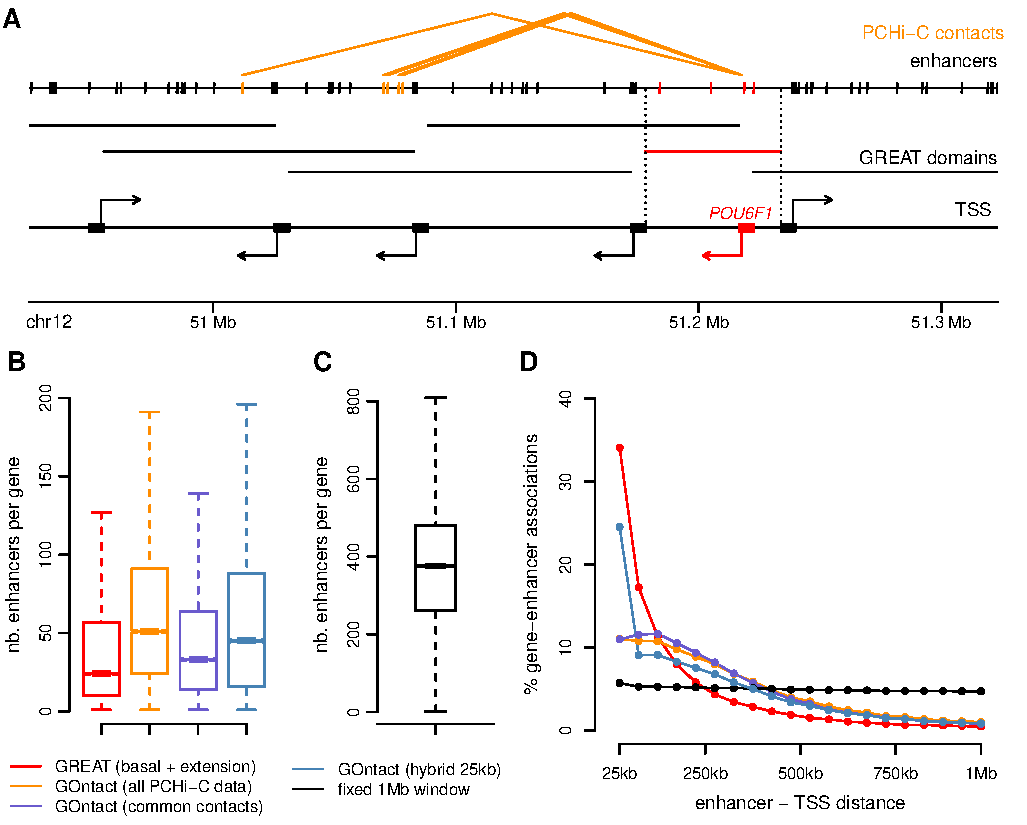
\includegraphics[width=1\textwidth, page=1] {figures/GOntact/Figure1.pdf}
 \caption[Regulatory relationships between enhancers and gene.]{
 \textbf{Regulatory relationships between enhancers and gene.}
 \textbf{A.} Illustration of the enhancer target gene predictions that underlie functional enrichment analyses in GREAT and GOntact, in a 400 kb genomic region around the human \textit{POU6F1} gene. Top: rectangles indicate the positions of ENCODE-predicted enhancers, orange lines indicate chromatin contacts between the \textit{POU6F1} gene promoter and enhancers. Middle: horizontal segments represent extended regulatory domains (up to the neighboring genes’ basal domains, within a maximum distance of 1Mb from the canonical TSS) used in GREAT. The regulatory domain and the enhancers attributed to \textit{POU6F1} by GREAT are depicted in red. Bottom: arrows depict the positions and the orientations of canonical transcription start sites (TSS) for \textit{POU6F1} and neighboring genes; black rectangles depict basal gene regulatory domains (5kb upstream, 1kb downstream of TSS) used in the default GREAT implementation. 
 \textbf{B.} Boxplots representing the numbers of enhancers assigned to genes with GREAT, with GOntact (orange: using all available PCHi-C data; purple: using chromatin contacts shared across at least 2 PCHi-C samples) or with the hybrid GOntact-GREAT approach (Methods). 
 \textbf{C.} Boxplot representing the numbers of enhancers attributed to genes with a fixed window approach (1Mb around the TSS; Methods). 
 \textbf{D.} Distribution of the distances between genes and enhancers predicted to be in regulatory interactions with the GREAT, GOntact or fixed window approach. Color code as in B and C.
 \\
 }
 \label{fig:GOntact-fig1}
\end{figure} 

The genomic distances between promoters and enhancers predicted to be in regulatory interactions vary considerably among methods. With GREAT, 51\% of all gene-enhancer pairs are separated by less than 100 kb and 8\% are separated by more than 500 kb (Figure \ref{fig:GOntact-fig1}.D). With GOntact, distances between pairs of enhancers and promoters are generally larger: only 22\% are separated by less than 100 kb, and 16\% are separated by more than 500 kb (Figure \ref{fig:GOntact-fig1}.D). We note that there is an excess of enhancers situated within 50 kb of the TSS even when we define gene-enhancer pairs with a “fixed window” approach, that is, when we assign to genes all enhancers present within a maximum distance of 1 Mb of the TSS (Figure \ref{fig:GOntact-fig1}.D). In contrast, regulatory associations inferred from PCHi-C data are less frequent in close proximity to genes, which is at least in part due to the technical difficulty of distinguishing genuine from spurious chromatin contacts at small distances on the linear genome \citep{cairns_chicago_2016}. To compensate for this, we combined the principles of GREAT and GOntact into a "hybrid" method: each gene is assigned a basal regulatory domain (comprising for example 25 kb upstream and 25 kb downstream of the TSS), as well as all enhancers that are in contact with its promoters in the PCHi-C data. The promoter-enhancer distance distribution for this “hybrid” approach combines features of GREAT and GOntact, as expected (Figure \ref{fig:GOntact-fig1}.D)


\subsection{Gene ontology enrichment tests}

Beyond defining putative target genes for \gls{cis}-regulatory elements, the aim of both GOntact and GREAT is to test for the enrichment of functional annotations associated with a set of \gls{cis}-regulatory elements. Here, we apply both methods to search for enrichments of Gene Ontology (GO) annotations, in a set of enhancers. With both approaches, each enhancer is assigned all GO categories that are associated with its predicted target genes. For each GO category, we then compute the proportion of enhancers that are associated with it, among all enhancers in the dataset of interest (hereafter termed “foreground set”). We then test for an enrichment by comparing this proportion with the proportion of enhancers associated with the same GO category within a background set of elements, with a one-sided binomial test (Methods). This procedure is identical to the one implemented in GREAT, the only difference resides in the target gene assignment for enhancers. We note however that the default behavior in GREAT (at least in the web server version) is to estimate the proportion of elements associated by chance with a GO category as the cumulative size of all regulatory domains of genes that have this GO annotation, relative to the total size of the genome \citep{mclean_great_2010}. Here, we prefer to define the proportion expected by chance using a background set of enhancers, for better comparability between GREAT and GOntact. In the examples shown here, we used as a background the full set of ENCODE-predicted enhancers, which consists of 408737 elements for human and 739996 elements for mouse \citep{davis_encyclopedia_2018,laverre_long-range_2022}. As these datasets were obtained using a large number of cell types, tissues and biological conditions, we reasoned that they can provide a good estimation of what is expected at the genome-wide level for enhancer elements. 

\subsection{GOntact and GREAT functional annotations are coherent with enhancer activity patterns}

We applied GREAT and GOntact on sets of experimentally validated enhancers for human and mouse, downloaded from the Vista Enhancer Browser \citep{visel_vista_2007}. We analyzed sets of enhancers that are active in the embryonic heart and in the embryonic midbrain (141 and 279 enhancers for human, 170 and 166 enhancers for mouse, respectively). We evaluated GO enrichments with 5 method variations: the GREAT default “basal+extension” approach, the fixed window approach (each gene is assigned all enhancers found within a maximum 1Mb distance of its TSS), GOntact using all available PCHi-C data, GOntact using chromatin contacts observed in at least 2 PCHi-C samples and the GOntact - GREAT hybrid approach (each gene is attributed a basal regulatory domain consisting of 25 kb upstream and downstream of TSS + all enhancers in PCHi-C-defined contact with its promoter). \\

We found that all 5 methods yielded GO enrichment results that were coherent with the patterns of activity of the input enhancer datasets. For example, for embryonic heart enhancers, all methods reveal significant enrichments for GO categories related to muscle functions (Figures \ref{fig:GOntact-fig2}, \ref{fig:GOntact-fig3}). Likewise, for embryonic midbrain enhancers, all 5 methods reveal significant GO enrichments related to neural differentiation (Figures \ref{fig:GOntact-fig2}, \ref{fig:GOntact-fig3}). Although there is considerable overlap between the significant GO categories found by all methods (Figure \ref{fig:GOntact-fig4}.), each of them appears to prioritize a different subset of biologically relevant GO annotations. For example, for embryonic heart enhancers, GOntact methods tend to bring forward categories related to the early development of the organ (e.g., lateral mesoderm formation, embryonic heart tube elongation), whereas GREAT seems to prioritize categories related to the physiology of the embryonic and adult organ, such as the regulation of striated muscle contraction or the regulation of blood circulation (Figures \ref{fig:GOntact-fig2}, \ref{fig:GOntact-fig3}). Interestingly, for embryonic midbrain enhancers, both GREAT and GOntact find stronger enrichments for processes related to gene expression regulation, rather than to brain development (Figures \ref{fig:GOntact-fig2}, \ref{fig:GOntact-fig3}).

\begin{figure}[hbt!]
 \centering
 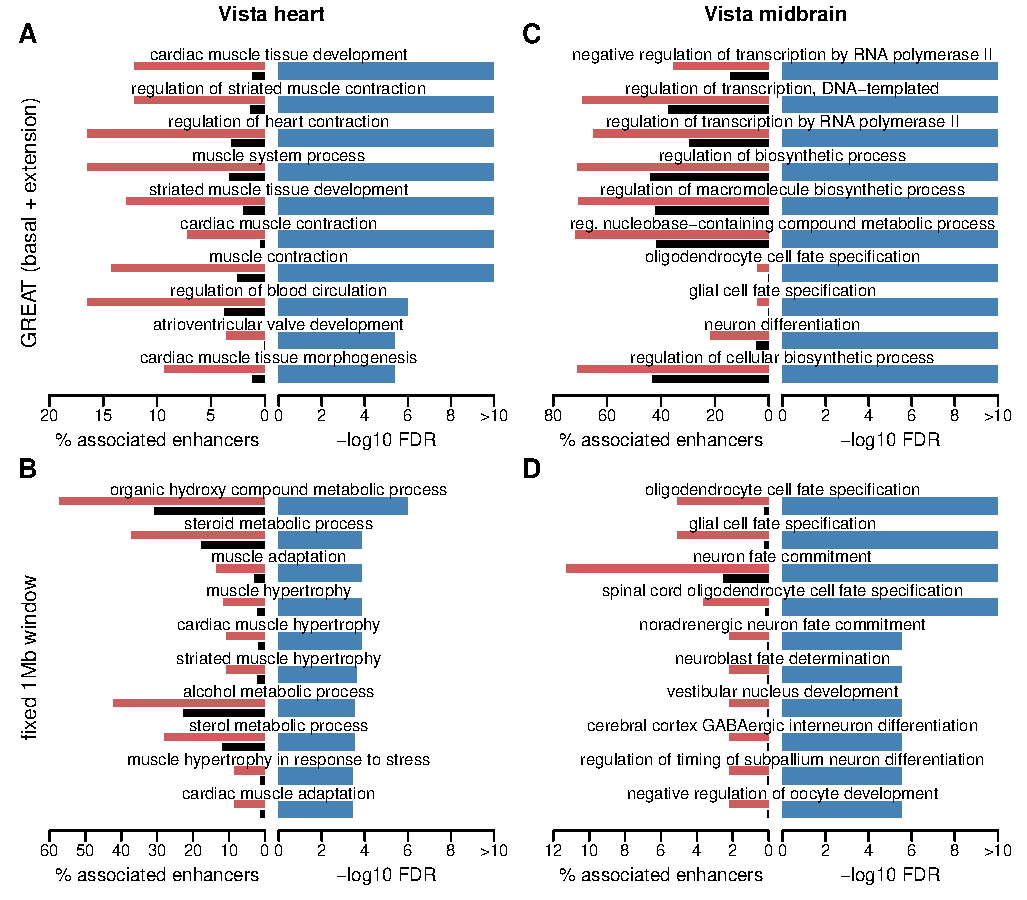
\includegraphics[width=1\textwidth, page=1] {figures/GOntact/Figure2.pdf}
 \caption[Gene Ontology Enrichment from neighboring association.]{
 \textbf{Gene Ontology Enrichment from neighboring association.}
 \textbf{A.} Gene Ontology categories that are significantly enriched (FDR $<$ 0.05, minimum enrichment 1.5, Methods) in a GREAT analysis of 141 experimentally validated human enhancers that are active in the embryonic heart (Vista), compared with a background consisting of the entire set of ENCODE-predicted enhancers. GREAT was run with default parameters: basal regulatory domain (5 kb upstream of TSS, 1 kb downstream of TSS) and an extension of a maximum 1 Mb. 
 \textbf{B.} Same as A, where enhancers are attributed to genes with a fixed 1Mb window approach (Methods). 
 \textbf{C, D.} Same as A, B for a set of 279 experimentally validated human enhancers that are active in the embryonic midbrain. 
 \\
 }
 \label{fig:GOntact-fig2}
\end{figure} 

\begin{figure}[hbt!]
 \centering
 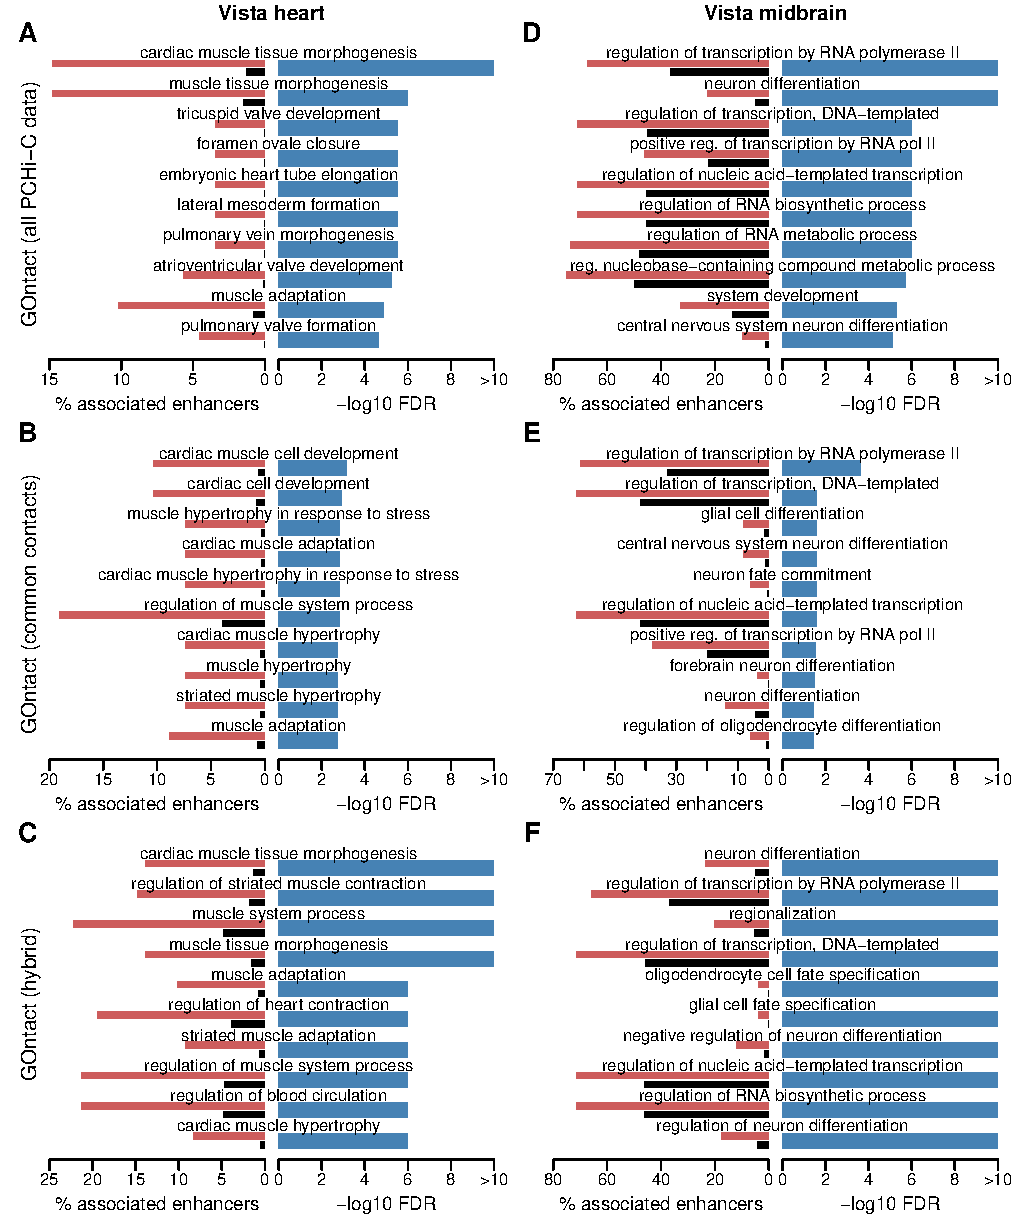
\includegraphics[width=1\textwidth, page=1] {figures/GOntact/Figure3.pdf}
 \caption[Gene Ontology Enrichment from chromatin contacts.]{
 \textbf{Gene Ontology Enrichment from chromatin contacts.}
 \textbf{A.} Gene Ontology categories that are significantly enriched (FDR $<$ 0.05, minimum enrichment 1.5, Methods) in a GOntact analysis of 141 experimentally validated human enhancers that are active in the embryonic heart (Vista), compared with a background consisting of the entire set of ENCODE-predicted enhancers. GOntact was run with all available PCHi-C data (N interactions) and a maximum distance of 1Mb was set for interactions.
 \textbf{B.} Same as A, where GOntact was run using only those interactions observed in at least 2 PCHi-C samples (N=). 
 \textbf{C.} Same as A, where GOntact was run in hybrid mode (basal domain of 25 kb upstream and downstream of TSS + chromatin contacts derived from all PCHi-C samples). 
 \textbf{D, E, F.} Same as A, B, C, for a set of 279 experimentally validated human enhancers that are active in the embryonic midbrain. 
 \\
 }
 \label{fig:GOntact-fig3}
\end{figure} 

\subsection{Enrichment of meaningful functional annotations with a simple “fixed window” approach}

Surprisingly, the simplest method used in the assignment of putative enhancer target genes (the fixed 1 Mb window approach) also reveals numerous biologically relevant GO category enrichments, at least with the enhancer datasets that we tested (Figure \ref{fig:GOntact-fig2}.). For heart enhancers, this approach reveals significant enrichments for metabolic processes, but also for muscle adaptation and muscle hypertrophy (Figure \ref{fig:GOntact-fig2}.). In fact, for this set of human enhancers, the fixed window approach is the most sensitive: it uniquely identifies more than 300 significantly enriched GO categories that are not shared with the other approaches (Figure \ref{fig:GOntact-fig4}.A). However, we note that these GO categories tend to be more general than the ones identified by the other approaches, as they are associated with a much higher proportion of background enhancers (Figure \ref{fig:GOntact-fig4}.C). For brain enhancers, the fixed window approach finds enrichments for GO categories related to the differentiation and commitment of various brain cell types (oligodendrocytes, glial cells, neurons). In this case, the fixed window approach identifies fewer significant GO categories than the other approaches, but these categories tend to be more specific than the ones identified by the other 4 approaches, as they are associated with smaller proportions of background enhancers (Figure \ref{fig:GOntact-fig4}.D).

\begin{figure}[hbt!]
 \centering
 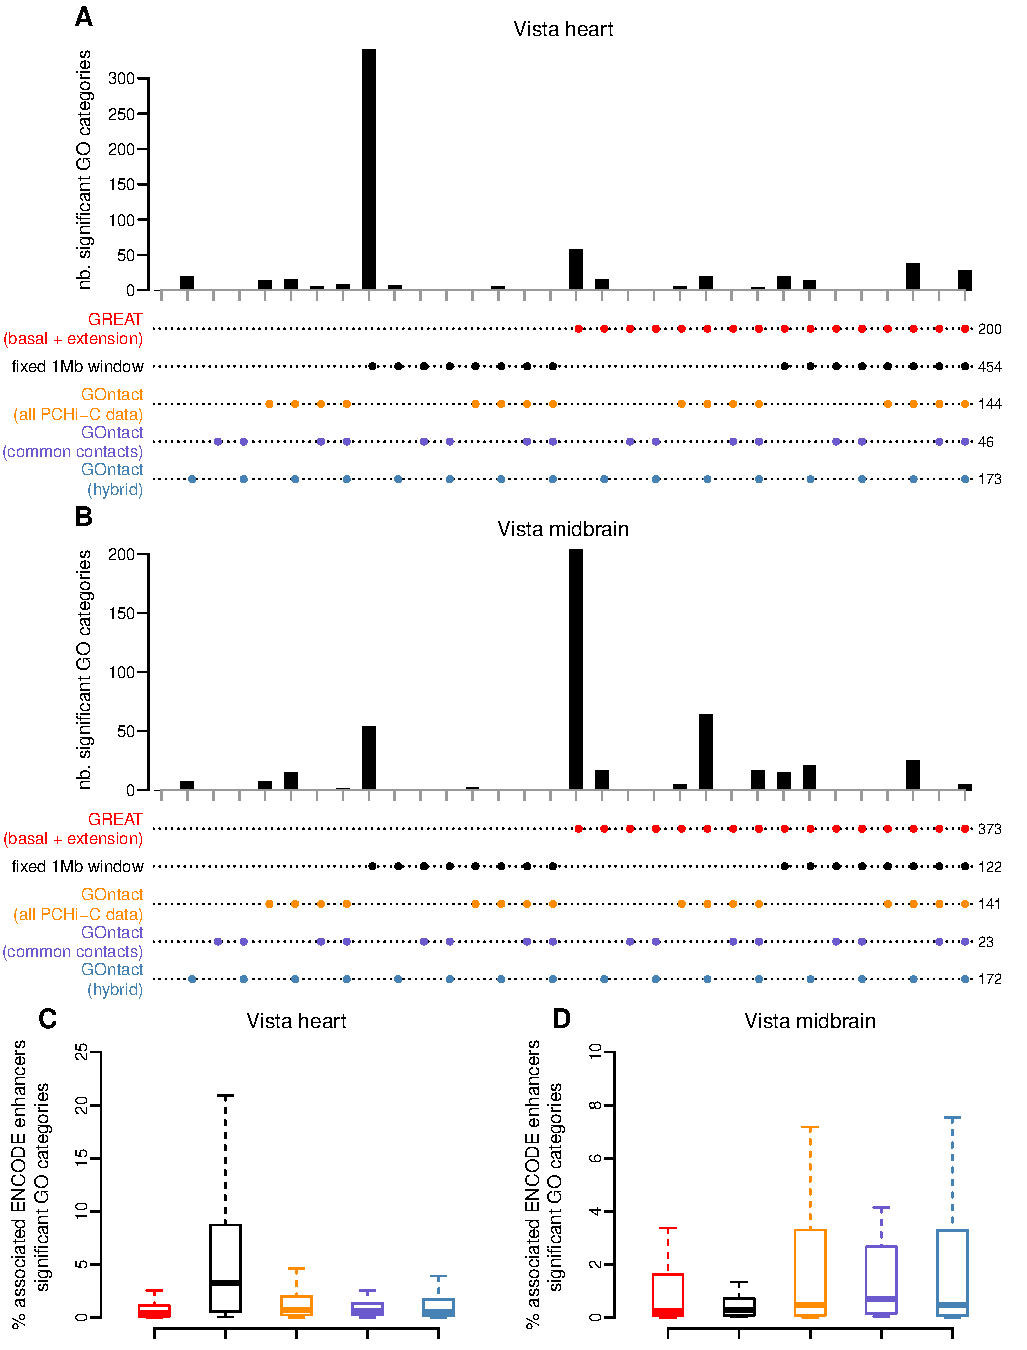
\includegraphics[width=0.8\textwidth, page=1] {figures/GOntact/Figure4.pdf}
 \caption[Comparison between Gene Ontology enrichment results obtained with different methods]{
 \textbf{Comparison between Gene Ontology enrichment results obtained with different methods :}
 \textbf{A.} GREAT (default implementation, red), fixed window (black), GOntact (using all PCHi-C data, dark orange), GOntact (using chromatin contacts observed in at least 2 PCHi-C samples, purple), GOntact hybrid mode (25 kb fixed window around TSS + chromatin contacts from all PCHi-C data, blue). The bars represent the number of significantly enriched GO categories (maximum FDR 0.05, minimum enrichment 1.5) in the 32 possible combinations of the 5 cited methods. The colored dots below the bars represent for each method whether it was included in each combination. The enrichment was computed by comparing a set of 141 experimentally validated human enhancers active in the heart with the entire ENCODE enhancer dataset. 
 \textbf{B.} Same as A, for 279 enhancers active in the brain. 
 \textbf{C.} Boxplots depicting the proportions of ENCODE enhancers that are associated with each significantly enriched GO category, detected with the 5 methods described above. 
 \textbf{D.} Same as C, for 279 enhancers active in the brain. 
 \\
 }
 \label{fig:GOntact-fig4}
\end{figure} 

\subsection{GOntact variants that increase sensibility and specificity}
In the default implementation of GOntact, only PCHi-C contacts are used to infer enhancer target genes. Because interactions at short genomic distances are depleted in chromatin contact data, and because there is a genuine enrichment for regulatory elements in close proximity to the gene promoter \citep{gasperini_genome-wide_2019}, we decided to combine the principles used in the two methods into a hybrid GOntact-GREAT approach. With this approach, each gene is assigned a proximal regulatory domain (for example, 25 kb upstream and 25 kb downstream of the TSS), and all enhancers found in this domain are attributed to the corresponding gene. In addition, we add all enhancers that are connected to the gene promoter through chromatin contacts, in cis, within a maximum genomic distance (by default equal to 1 Mb). This approach efficiently combines the characteristics of GREAT and GOntact, both in terms of the distances between promoters and enhancers that are part of the inferred regulatory pairs (Figure \ref{fig:GOntact-fig1}.D), and in terms of the Gene Ontology enrichments that can be detected (Figures 2-4). The numbers of significantly enriched GO categories are indeed intermediate in the hybrid approach compared to GREAT and GOntact (Figure \ref{fig:GOntact-fig4}.) and are also coherent with the expression patterns of the selected sets of enhancers (Figure \ref{fig:GOntact-fig3}.).\\

A key factor for the success of the GOntact approach is evidently the input PCHi-C data. Ideally, chromatin contacts and \gls{cis}-regulatory element activity should be assessed in the same biological conditions. However, PCHi-C data is not yet available or efficiently produced for many cell types or tissues. As an alternative, we used the subset of chromatin interactions that were detected in at least two PCHi-C samples (Methods). This restricted set of interactions should be enriched in widespread (or even ubiquitous) chromatin contacts, which are likely relevant for the regulatory program of the tissue or cell type in which enhancer activity was assayed. A disadvantage is that the number of interactions that can be used is substantially reduced, which likely affects our power to detect statistically significant functional enrichments. Indeed, we found much fewer significantly enriched GO categories with this conservative variant of GOntact than with all available PCHi-C data or with the GREAT approach (Figure \ref{fig:GOntact-fig4}.). However, these functional annotations remain biologically relevant: biological processes related to cardiac cell development and muscle adaptation were found for the embryonic heart enhancers (Figure \ref{fig:GOntact-fig3}.B), and categories related to neural cell differentiation were identified for the embryonic brain (Figure \ref{fig:GOntact-fig3}.E). 

\section{Discussion}
Both GOntact and GREAT aim to predict putative biological functions for a set of \gls{cis}-regulatory elements of gene expression. This functional annotation can serve as a basis for further experimental validations, and can thus be seen as a source of testable hypotheses. We are indeed unable to perfectly assess the validity of our results because we lack a “golden truth”. Instead, we can only judge whether the results that we obtain are biologically meaningful, given what is known about the input dataset. Here, we applied our methods on sets of experimentally validated enhancer elements, whose pattern of activity was ascertained in mouse embryos with enhancer trap experiments \citep{visel_vista_2007}. We thus expect an enrichment for biological processes associated with the development and the physiology of the organs in which enhancer activity was detected. Reassuringly, all the methods that we tested here show results that are coherent with these expectations, at least to some extent. \\

GOntact and GREAT generally provide consistent Gene Ontology enrichment results, which is somewhat surprising given that these two methods rely on very different approaches for target gene inference. In GREAT, regulatory relationships between genes and enhancers are inferred by defining a regulatory domain for each gene, which basically always includes a proximal domain around the canonical gene TSS, and which can extend no further than the TSS of the neighboring genes, within a certain maximum genomic distance. The main assumption here is that enhancers generally regulate their neighboring genes. In GOntact, regulatory relationships are inferred based on the presence of chromatin contacts that involve gene promoters and enhancers. Thus, while GREAT only relies on the existing gene annotations to infer regulatory relationships, in GOntact we use direct experimental evidence supporting the physical proximity between promoters and enhancers. We thus expect to have a better-informed prediction of enhancer target genes, in light of the accumulating evidence that gene expression regulation is often achieved through the formation of chromatin contacts that bring promoters and distal elements in physical proximity in the nucleus \citep{lettice_long-range_2003, sagai_elimination_2005, schoenfelder_pluripotent_2015, mifsud_mapping_2015,javierre_lineage-specific_2016, schoenfelder_long-range_2019}. However, we note that although chromatin contacts detected with PCHi-C are enriched in probable regulatory relationships \citep{schoenfelder_pluripotent_2015,mifsud_mapping_2015}, they are not restricted to this type of interaction. The chromatin contact datasets that we used as an input for GOntact are likely to include false positives arising as artifacts of the computational or biochemical methodologies that were employed, as well as genuine chromatin contacts that are not involved in gene expression regulation. Despite these drawbacks, we believe that GOntact nevertheless provides a useful alternative to the regulatory relationships inferred by the classical “genomic proximity” approach implemented in GREAT. \\

A major advantage of the regulatory relationships inferred by GOntact is that they are to a large extent independent of the genome organization, in contrast with the methods implemented in GREAT. The definition of the regulatory domains directly depends on the TSS coordinates of the neighboring genes, upstream and downstream of the gene of interest. The quality of genomic annotations is thus a major confounding factor in the inference of regulatory relationships. A missing gene or a wrongly assigned transcription start site can have an inordinate impact on the definition of other genes’ regulatory domains. At least in well-assembled and well-annotated genomes such as human and mouse, GREAT nevertheless seems to perform extremely well, in that it generates functional predictions that are perfectly coherent with the patterns of activity of enhancer elements. Part of the success of the method may be explained by the fact that a large proportion of regulatory elements are indeed situated in close genomic proximity to the TSS of the gene they regulate. Although GREAT likely misses more distant regulatory elements, situated beyond the TSS of the neighboring genes, the fact that it perfectly captures proximal regulatory elements can be sufficient to detect enriched functions in any given set of enhancers. We propose that the same mechanism can explain the unexpected success of the simplest approach used in this study, the “fixed window” method in which enhancers are attributed to all genes whose TSS are closer than a certain distance threshold (here 1Mb). \\

While GREAT is dependent on genomic organization and on genomic annotations in general, GOntact is also likely dependent on the quantity, quality and specificity of the input data, namely the set of PCHi-C chromatin contacts. In the default GOntact implementation, we propose using a previously published set of chromatin interactions, derived from multiple cell types and conditions. A non-negligible fraction of these interactions are cell type-specific \citep{javierre_lineage-specific_2016, laverre_long-range_2022}, and these interactions do not necessarily provide useful information for the functional annotations of sets of enhancers that are active in other cell types or tissues. Ideally, chromatin interactions should be provided for the same biological conditions (tissues, cell types, developmental stages etc.) in which \gls{cis}-regulatory element activity is assessed. In the absence of perfectly matched chromatin contact and enhancer activity data, a convenient solution is to use as an input a set of chromatin interactions that are shared across multiple biological conditions, which are thus likely to be relevant in the biological context that is being examined. This filter greatly reduces the number of usable interactions and thus results in a decrease in sensitivity, but also likely reduces the frequency of false positives. With the increasing availability of high-resolution chromatin contact data, we believe that GOntact can provide good functional predictions for \gls{cis}-regulatory elements. We particularly recommend using GOntact for biological contexts where long-range regulatory relationships are known to be frequent, for example in developing mammalian tissues \citep{de_laat_topology_2013}. 


\section{Methods}
\subsection*{Promoter Capture Hi-C data}
We retrieved processed PCHi-C data from a previous study, which processed and combined 26 human and 14 mouse samples \citep{laverre_long-range_2022}. The PCHi-C data selected in this study was all generated with the same protocol, ensuring its comparability across samples. The PCHi-C technique aims to identify chromatin contacts between a predefined set of restriction fragments, that are “baited” using RNA molecules, and the entire genome. Baited fragments were designed to target gene promoters \citep{mifsud_mapping_2015, schoenfelder_pluripotent_2015}. All chromatin interactions present in this data involve at least one baited restriction fragment. Interactions were scored using the HiCup and ChICAGO tools, on the hg38 and mm10 genome assemblies for human and mouse, respectively \citep{wingett_hicup:_2015,cairns_chicago_2016}. 

\subsection*{Genome annotations}
We used BioMart to download gene annotations from the Ensembl database release 102, for human hg38 and mouse mm10 genome assemblies. For each annotated gene and transcript, we extracted the gene identifier and gene symbol, the genomic coordinates of the transcription start sites (TSS), the exonic length and the APPRIS isoform annotation. We determined the major isoform for each protein-coding gene using its APPRIS annotation: transcripts with the “principal1” tag were preferred, followed by “principal2” transcripts if the former were not available, and so on. If no APPRIS annotations were available, the major isoform was defined as the one with the longest exonic length. 

\subsection*{Bait annotations}
We analyzed the overlap between baited restriction fragments and protein-coding gene transcription start sites, using the coordinates of the major isoforms defined above. Baits were attributed to all genes whose transcription start sites overlapped with or were within at most 1 kb of the bait coordinates. 

\subsection*{Gene Ontology annotations}
We downloaded Gene Ontology (GO) annotations for human and mouse from geneontology.org, for the 2021-11-16 database release. For human we used Gene Ontology annotations generated by UniProt on 2021-11-08 and for mouse we used annotations generated by Mouse Genome Informatics on 2021-11-15. Genes were associated with Gene Ontology categories through their symbol or usual name. We also downloaded the descriptions and hierarchical relationships between Gene Ontology categories in Obo format. Gene Ontology annotations are provided only for the most precise term of a given ontology “branch”, but genes are assumed to inherit the annotations of all the parent terms. We processed Gene Ontology data within the GOntact software to propagate gene annotations through the term hierarchy. Following the procedure implemented in GREAT, for all analyses performed here we considered only those genes that had at least one Gene Ontology annotation. In the analyses presented in the manuscript, we focused on the “biological process” Gene Ontology domain. Results for the “molecular function” and “cellular component” domains are provided in the supplementary materials. 


\subsection*{Target gene inference for cis-regulatory elements with GREAT}
To ensure perfect comparability between methods, we reimplemented the GREAT approach as described by the authors, using the genomic and Gene Ontology annotations described above. We focused on the default method for enhancer-target gene associations, namely, the “basal + extension” approach. The parameters for the basal and extended domains definition are command-line arguments in GOntact and can thus be chosen by the user. Here we used the default parameters used in the GREAT web server, that is, a basal domain consisting of 5 kb upstream and 1 kb downstream of the TSS and an extension of maximum 1 Mb. Each gene is thus attributed a basal regulatory domain and domains are extended in both directions up to the basal domains of the neighboring genes, within the maximum distance defined above. Enhancers found within each regulatory domain are attributed to the corresponding genes. 

\subsection*{Target gene inference for cis-regulatory elements with a fixed window approach}
We also implemented a simple distance-based assignment of putative target genes for enhancers, with a fixed window approach. With this approach, each gene is assigned all enhancers found within a maximum distance of its TSS, upstream or downstream. We used a maximum distance of 1 Mb, as for the other methods implemented here. In practice, this approach is available using the GREAT mode in GOntact, by defining a basal regulatory domain with size of 1 Mb upstream and downstream of the TSS and an extension of 0. 

\subsection*{Target gene inference for cis-regulatory elements with GOntact}
To infer enhancer target genes using chromatin contact data, we first analyzed the overlap and the distance between enhancer coordinates and restriction fragments. We used only interactions involving a baited (promoter) and an unbaited restriction fragment, in cis, within a maximum distance of 1 Mb. An enhancer is said to be in chromatin contact with a baited promoter if it overlaps with or if it is found within a certain maximum distance of the restriction fragments that interact with the baited fragment. The maximum distance between enhancers and restriction fragments is a command-line argument of the GOntact program and with a default value of 5 kb. 

\subsection*{Gene Ontology enrichment tests}
To infer significant enrichments of Gene Ontology annotations, we compare a foreground set of enhancers with a background set of enhancers. Here we used as background the ENCODE sets of enhancers for human and mouse. Each enhancer is assigned all Gene Ontology categories that are associated with its putative target genes. For each set of enhancers and for each Gene Ontology category, we can thus compute the proportion of enhancers associated with it. We then compare the proportions observed in the foreground and in the background set with an one-sided binomial test. False discovery rates (FDR) are computed with the Benjamini-Hochberg procedure.

\subsection*{Code and data availability}
All methods described here were implemented in a package named GOntact, written in OCaml. The source code and the R scripts used to generate graphics and statistical analyses are freely available in a GitLab repository: 
https://gitlab.in2p3.fr/anamaria.necsulea/GOntact
For reproducibility, we provide all data, source code and program binaries in a Singularity image. Processed data and supplementary files are also available here:

http://pbil.univ-lyon1.fr/members/necsulea/GOntact 


\subsection*{Acknowledgements}
We thank C. Berthelot, Y. Ghavi-Helm, F. Picard, C. François and D. Mouchiroud for discussions and advice on the project. Computational analyses were performed using the computing facilities of the CC LBBE/PRABI and the Core Cluster of the Institut Français de Bioinformatique (IFB) (ANR-11-INBS-0013). This work was funded by the French National Research Agency (ANR-17-CE12-0019-01 «LncEvoSys»). 
